%
% Generated on matcha.io
%


\tikzset{every picture/.style={line width=0.75pt}} %set default line width to 0.75pt        

\begin{center}
    

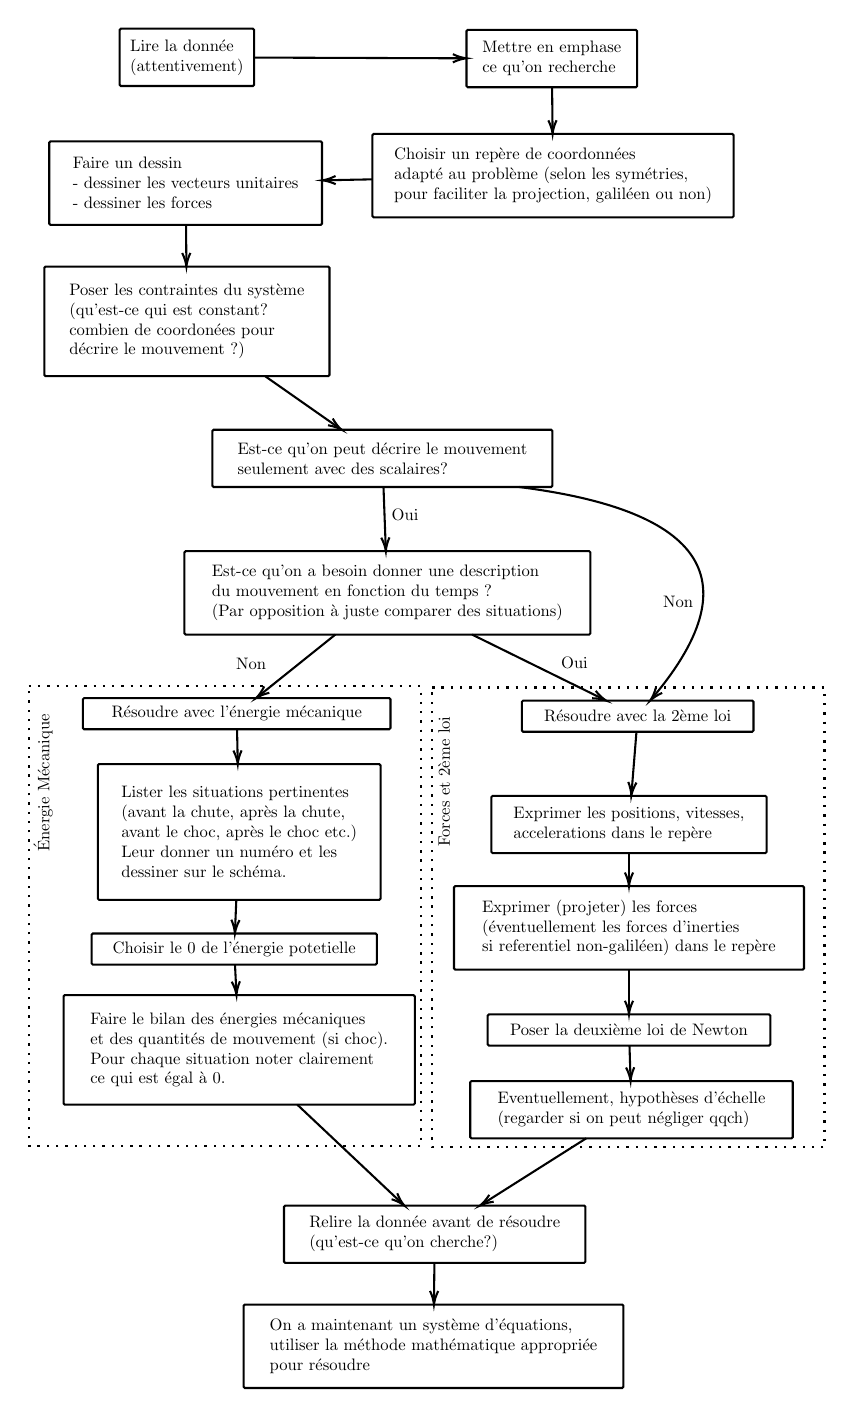
\begin{tikzpicture}[x=0.75pt,y=0.75pt,yscale=-.6,xscale=.6, every node/.style={scale=0.6}]]
    %uncomment if require: \path (0,1260); %set diagram left start at 0, and has height of 1260
    
    %Shape: Rectangle [id:dp4576841307529028] 
    \draw  [dash pattern={on 0.84pt off 2.51pt}] (26,567) -- (341,567) -- (341,936) -- (26,936) -- cycle ;
    %Shape: Rectangle [id:dp5066185054013125] 
    \draw  [dash pattern={on 0.84pt off 2.51pt}] (350,568) -- (665,568) -- (665,937) -- (350,937) -- cycle ;
    
    % Text Node
    \draw    (99.02,40) .. controls (99.02,39.45) and (99.47,39) .. (100.02,39) -- (206.02,39) .. controls (206.58,39) and (207.02,39.45) .. (207.02,40) -- (207.02,84) .. controls (207.02,84.55) and (206.58,85) .. (206.02,85) -- (100.02,85) .. controls (99.47,85) and (99.02,84.55) .. (99.02,84) -- cycle  ;
    \draw (153.02,62) node   [align=left] {Lire la donnée\\(attentivement)};
    % Text Node
    \draw    (377.52,41) .. controls (377.52,40.45) and (377.97,40) .. (378.52,40) -- (513.52,40) .. controls (514.08,40) and (514.52,40.45) .. (514.52,41) -- (514.52,85) .. controls (514.52,85.55) and (514.08,86) .. (513.52,86) -- (378.52,86) .. controls (377.97,86) and (377.52,85.55) .. (377.52,85) -- cycle  ;
    \draw (446.02,63) node   [align=left] {Mettre en emphase\\ce qu'on recherche};
    % Text Node
    \draw    (302.02,124.5) .. controls (302.02,123.95) and (302.47,123.5) .. (303.02,123.5) -- (591.02,123.5) .. controls (591.58,123.5) and (592.02,123.95) .. (592.02,124.5) -- (592.02,189.5) .. controls (592.02,190.05) and (591.58,190.5) .. (591.02,190.5) -- (303.02,190.5) .. controls (302.47,190.5) and (302.02,190.05) .. (302.02,189.5) -- cycle  ;
    \draw (447.02,157) node   [align=left] {Choisir un repère de coordonnées \\adapté au problème (selon les symétries, \\pour faciliter la projection, galiléen ou non)};
    % Text Node
    \draw    (42.52,130.5) .. controls (42.52,129.95) and (42.97,129.5) .. (43.52,129.5) -- (260.52,129.5) .. controls (261.08,129.5) and (261.52,129.95) .. (261.52,130.5) -- (261.52,195.5) .. controls (261.52,196.05) and (261.08,196.5) .. (260.52,196.5) -- (43.52,196.5) .. controls (42.97,196.5) and (42.52,196.05) .. (42.52,195.5) -- cycle  ;
    \draw (152.02,163) node   [align=left] {Faire un dessin\\\mbox{-} dessiner les vecteurs unitaires\\\mbox{-} dessiner les forces};
    % Text Node
    \draw    (38.52,231) .. controls (38.52,230.45) and (38.97,230) .. (39.52,230) -- (266.52,230) .. controls (267.08,230) and (267.52,230.45) .. (267.52,231) -- (267.52,317) .. controls (267.52,317.55) and (267.08,318) .. (266.52,318) -- (39.52,318) .. controls (38.97,318) and (38.52,317.55) .. (38.52,317) -- cycle  ;
    \draw (153.02,274) node   [align=left] {Poser les contraintes du système\\(qu'est-ce qui est constant?\\combien de coordonées pour\\décrire le mouvement ?)};
    % Text Node
    \draw    (173.52,362) .. controls (173.52,361.45) and (173.97,361) .. (174.52,361) -- (445.52,361) .. controls (446.08,361) and (446.52,361.45) .. (446.52,362) -- (446.52,406) .. controls (446.52,406.55) and (446.08,407) .. (445.52,407) -- (174.52,407) .. controls (173.97,407) and (173.52,406.55) .. (173.52,406) -- cycle  ;
    \draw (310.02,384) node   [align=left] {Est-ce qu'on peut décrire le mouvement\\seulement avec des scalaires?};
    % Text Node
    \draw    (151.02,459.5) .. controls (151.02,458.95) and (151.47,458.5) .. (152.02,458.5) -- (476.02,458.5) .. controls (476.58,458.5) and (477.02,458.95) .. (477.02,459.5) -- (477.02,524.5) .. controls (477.02,525.05) and (476.58,525.5) .. (476.02,525.5) -- (152.02,525.5) .. controls (151.47,525.5) and (151.02,525.05) .. (151.02,524.5) -- cycle  ;
    \draw (314.02,492) node   [align=left] {Est-ce qu'on a besoin donner une description\\du mouvement en fonction du temps ?\\(Par opposition à juste comparer des situations)};
    % Text Node
    \draw (316,423) node [anchor=north west][inner sep=0.75pt]   [align=left] {Oui};
    % Text Node
    \draw    (69.52,577.5) .. controls (69.52,576.95) and (69.97,576.5) .. (70.52,576.5) -- (315.52,576.5) .. controls (316.08,576.5) and (316.52,576.95) .. (316.52,577.5) -- (316.52,600.5) .. controls (316.52,601.05) and (316.08,601.5) .. (315.52,601.5) -- (70.52,601.5) .. controls (69.97,601.5) and (69.52,601.05) .. (69.52,600.5) -- cycle  ;
    \draw (193.02,589) node   [align=left] {Résoudre avec l'énergie mécanique};
    % Text Node
    \draw (191,543) node [anchor=north west][inner sep=0.75pt]   [align=left] {Non};
    % Text Node
    \draw    (422.02,579.5) .. controls (422.02,578.95) and (422.47,578.5) .. (423.02,578.5) -- (607.02,578.5) .. controls (607.58,578.5) and (608.02,578.95) .. (608.02,579.5) -- (608.02,602.5) .. controls (608.02,603.05) and (607.58,603.5) .. (607.02,603.5) -- (423.02,603.5) .. controls (422.47,603.5) and (422.02,603.05) .. (422.02,602.5) -- cycle  ;
    \draw (515.02,591) node   [align=left] {Résoudre avec la 2ème loi};
    % Text Node
    \draw (452,542) node [anchor=north west][inner sep=0.75pt]   [align=left] {Oui};
    % Text Node
    \draw (534,493) node [anchor=north west][inner sep=0.75pt]   [align=left] {Non};
    % Text Node
    \draw    (397.52,656) .. controls (397.52,655.45) and (397.97,655) .. (398.52,655) -- (617.52,655) .. controls (618.08,655) and (618.52,655.45) .. (618.52,656) -- (618.52,700) .. controls (618.52,700.55) and (618.08,701) .. (617.52,701) -- (398.52,701) .. controls (397.97,701) and (397.52,700.55) .. (397.52,700) -- cycle  ;
    \draw (508.02,678) node   [align=left] {Exprimer les positions, vitesses,\\accelerations dans le repère};
    % Text Node
    \draw    (367.52,728.5) .. controls (367.52,727.95) and (367.97,727.5) .. (368.52,727.5) -- (647.52,727.5) .. controls (648.08,727.5) and (648.52,727.95) .. (648.52,728.5) -- (648.52,793.5) .. controls (648.52,794.05) and (648.08,794.5) .. (647.52,794.5) -- (368.52,794.5) .. controls (367.97,794.5) and (367.52,794.05) .. (367.52,793.5) -- cycle  ;
    \draw (508.02,761) node   [align=left] {Exprimer (projeter) les forces\\(éventuellement les forces d'inerties \\si referentiel non-galiléen) dans le repère};
    % Text Node
    \draw    (394.52,831.5) .. controls (394.52,830.95) and (394.97,830.5) .. (395.52,830.5) -- (620.52,830.5) .. controls (621.08,830.5) and (621.52,830.95) .. (621.52,831.5) -- (621.52,854.5) .. controls (621.52,855.05) and (621.08,855.5) .. (620.52,855.5) -- (395.52,855.5) .. controls (394.97,855.5) and (394.52,855.05) .. (394.52,854.5) -- cycle  ;
    \draw (508.02,843) node   [align=left] {Poser la deuxième loi de Newton};
    % Text Node
    \draw    (231.02,985) .. controls (231.02,984.45) and (231.47,984) .. (232.02,984) -- (472.02,984) .. controls (472.58,984) and (473.02,984.45) .. (473.02,985) -- (473.02,1029) .. controls (473.02,1029.55) and (472.58,1030) .. (472.02,1030) -- (232.02,1030) .. controls (231.47,1030) and (231.02,1029.55) .. (231.02,1029) -- cycle  ;
    \draw (352.02,1007) node   [align=left] {Relire la donnée avant de résoudre\\(qu'est-ce qu'on cherche?)};
    % Text Node
    \draw    (380.52,885) .. controls (380.52,884.45) and (380.97,884) .. (381.52,884) -- (638.52,884) .. controls (639.08,884) and (639.52,884.45) .. (639.52,885) -- (639.52,929) .. controls (639.52,929.55) and (639.08,930) .. (638.52,930) -- (381.52,930) .. controls (380.97,930) and (380.52,929.55) .. (380.52,929) -- cycle  ;
    \draw (510.02,907) node   [align=left] {Eventuellement, hypothèses d'échelle\\(regarder si on peut négliger qqch)};
    % Text Node
    \draw    (81.52,630.5) .. controls (81.52,629.95) and (81.97,629.5) .. (82.52,629.5) -- (307.52,629.5) .. controls (308.08,629.5) and (308.52,629.95) .. (308.52,630.5) -- (308.52,737.5) .. controls (308.52,738.05) and (308.08,738.5) .. (307.52,738.5) -- (82.52,738.5) .. controls (81.97,738.5) and (81.52,738.05) .. (81.52,737.5) -- cycle  ;
    \draw (195.02,684) node   [align=left] {Lister les situations pertinentes\\(avant la chute, après la chute,\\avant le choc, après le choc etc.)\\Leur donner un numéro et les \\dessiner sur le schéma.};
    % Text Node
    \draw    (76.52,766.5) .. controls (76.52,765.95) and (76.97,765.5) .. (77.52,765.5) -- (304.52,765.5) .. controls (305.08,765.5) and (305.52,765.95) .. (305.52,766.5) -- (305.52,789.5) .. controls (305.52,790.05) and (305.08,790.5) .. (304.52,790.5) -- (77.52,790.5) .. controls (76.97,790.5) and (76.52,790.05) .. (76.52,789.5) -- cycle  ;
    \draw (191.02,778) node   [align=left] {Choisir le 0 de l'énergie potetielle};
    % Text Node
    \draw    (54.02,816) .. controls (54.02,815.45) and (54.47,815) .. (55.02,815) -- (335.02,815) .. controls (335.58,815) and (336.02,815.45) .. (336.02,816) -- (336.02,902) .. controls (336.02,902.55) and (335.58,903) .. (335.02,903) -- (55.02,903) .. controls (54.47,903) and (54.02,902.55) .. (54.02,902) -- cycle  ;
    \draw (195.02,859) node   [align=left] {Faire le bilan des énergies mécaniques\\et des quantités de mouvement (si choc).\\Pour chaque situation noter clairement \\ce qui est égal à 0.};
    % Text Node
    \draw    (198.52,1064.5) .. controls (198.52,1063.95) and (198.97,1063.5) .. (199.52,1063.5) -- (502.52,1063.5) .. controls (503.08,1063.5) and (503.52,1063.95) .. (503.52,1064.5) -- (503.52,1129.5) .. controls (503.52,1130.05) and (503.08,1130.5) .. (502.52,1130.5) -- (199.52,1130.5) .. controls (198.97,1130.5) and (198.52,1130.05) .. (198.52,1129.5) -- cycle  ;
    \draw (351.02,1097) node   [align=left] {On a maintenant un système d'équations,\\utiliser la méthode mathématique appropriée\\pour résoudre};
    % Text Node
    \draw (353.5,697.5) node [anchor=north west][inner sep=0.75pt]  [rotate=-270] [align=left] {Forces et 2ème loi};
    % Text Node
    \draw (28.5,701.5) node [anchor=north west][inner sep=0.75pt]  [rotate=-270] [align=left] {Énergie Mécanique};
    % Connection
    \draw    (207.02,62.18) -- (375.52,62.76) ;
    \draw [shift={(377.52,62.77)}, rotate = 180.2] [color={rgb, 255:red, 0; green, 0; blue, 0 }  ][line width=0.75]    (10.93,-3.29) .. controls (6.95,-1.4) and (3.31,-0.3) .. (0,0) .. controls (3.31,0.3) and (6.95,1.4) .. (10.93,3.29)   ;
    % Connection
    \draw    (446.27,86) -- (446.65,121.5) ;
    \draw [shift={(446.67,123.5)}, rotate = 269.39] [color={rgb, 255:red, 0; green, 0; blue, 0 }  ][line width=0.75]    (10.93,-3.29) .. controls (6.95,-1.4) and (3.31,-0.3) .. (0,0) .. controls (3.31,0.3) and (6.95,1.4) .. (10.93,3.29)   ;
    % Connection
    \draw    (302.02,159.95) -- (263.52,160.73) ;
    \draw [shift={(261.52,160.77)}, rotate = 358.83] [color={rgb, 255:red, 0; green, 0; blue, 0 }  ][line width=0.75]    (10.93,-3.29) .. controls (6.95,-1.4) and (3.31,-0.3) .. (0,0) .. controls (3.31,0.3) and (6.95,1.4) .. (10.93,3.29)   ;
    % Connection
    \draw    (152.33,196.5) -- (152.61,228) ;
    \draw [shift={(152.63,230)}, rotate = 269.48] [color={rgb, 255:red, 0; green, 0; blue, 0 }  ][line width=0.75]    (10.93,-3.29) .. controls (6.95,-1.4) and (3.31,-0.3) .. (0,0) .. controls (3.31,0.3) and (6.95,1.4) .. (10.93,3.29)   ;
    % Connection
    \draw    (310.88,407) -- (312.71,456.5) ;
    \draw [shift={(312.78,458.5)}, rotate = 267.88] [color={rgb, 255:red, 0; green, 0; blue, 0 }  ][line width=0.75]    (10.93,-3.29) .. controls (6.95,-1.4) and (3.31,-0.3) .. (0,0) .. controls (3.31,0.3) and (6.95,1.4) .. (10.93,3.29)   ;
    % Connection
    \draw    (215.82,318) -- (275.56,359.85) ;
    \draw [shift={(277.2,361)}, rotate = 215.02] [color={rgb, 255:red, 0; green, 0; blue, 0 }  ][line width=0.75]    (10.93,-3.29) .. controls (6.95,-1.4) and (3.31,-0.3) .. (0,0) .. controls (3.31,0.3) and (6.95,1.4) .. (10.93,3.29)   ;
    % Connection
    \draw    (272.23,525.5) -- (210.18,575.25) ;
    \draw [shift={(208.62,576.5)}, rotate = 321.28] [color={rgb, 255:red, 0; green, 0; blue, 0 }  ][line width=0.75]    (10.93,-3.29) .. controls (6.95,-1.4) and (3.31,-0.3) .. (0,0) .. controls (3.31,0.3) and (6.95,1.4) .. (10.93,3.29)   ;
    % Connection
    \draw    (382.04,525.5) -- (487.85,577.62) ;
    \draw [shift={(489.64,578.5)}, rotate = 206.22] [color={rgb, 255:red, 0; green, 0; blue, 0 }  ][line width=0.75]    (10.93,-3.29) .. controls (6.95,-1.4) and (3.31,-0.3) .. (0,0) .. controls (3.31,0.3) and (6.95,1.4) .. (10.93,3.29)   ;
    % Connection
    \draw    (419.68,407) .. controls (570.56,426.13) and (606.09,482.83) .. (526.24,577.08) ;
    \draw [shift={(525.03,578.5)}, rotate = 310.56] [color={rgb, 255:red, 0; green, 0; blue, 0 }  ][line width=0.75]    (10.93,-3.29) .. controls (6.95,-1.4) and (3.31,-0.3) .. (0,0) .. controls (3.31,0.3) and (6.95,1.4) .. (10.93,3.29)   ;
    % Connection
    \draw    (508.02,701) -- (508.02,725.5) ;
    \draw [shift={(508.02,727.5)}, rotate = 270] [color={rgb, 255:red, 0; green, 0; blue, 0 }  ][line width=0.75]    (10.93,-3.29) .. controls (6.95,-1.4) and (3.31,-0.3) .. (0,0) .. controls (3.31,0.3) and (6.95,1.4) .. (10.93,3.29)   ;
    % Connection
    \draw    (508.02,794.5) -- (508.02,828.5) ;
    \draw [shift={(508.02,830.5)}, rotate = 270] [color={rgb, 255:red, 0; green, 0; blue, 0 }  ][line width=0.75]    (10.93,-3.29) .. controls (6.95,-1.4) and (3.31,-0.3) .. (0,0) .. controls (3.31,0.3) and (6.95,1.4) .. (10.93,3.29)   ;
    % Connection
    \draw    (514.02,603.5) -- (510.03,653.01) ;
    \draw [shift={(509.87,655)}, rotate = 274.6] [color={rgb, 255:red, 0; green, 0; blue, 0 }  ][line width=0.75]    (10.93,-3.29) .. controls (6.95,-1.4) and (3.31,-0.3) .. (0,0) .. controls (3.31,0.3) and (6.95,1.4) .. (10.93,3.29)   ;
    % Connection
    \draw    (193.29,601.5) -- (193.83,627.5) ;
    \draw [shift={(193.88,629.5)}, rotate = 268.79] [color={rgb, 255:red, 0; green, 0; blue, 0 }  ][line width=0.75]    (10.93,-3.29) .. controls (6.95,-1.4) and (3.31,-0.3) .. (0,0) .. controls (3.31,0.3) and (6.95,1.4) .. (10.93,3.29)   ;
    % Connection
    \draw    (192.7,738.5) -- (191.64,763.5) ;
    \draw [shift={(191.56,765.5)}, rotate = 272.44] [color={rgb, 255:red, 0; green, 0; blue, 0 }  ][line width=0.75]    (10.93,-3.29) .. controls (6.95,-1.4) and (3.31,-0.3) .. (0,0) .. controls (3.31,0.3) and (6.95,1.4) .. (10.93,3.29)   ;
    % Connection
    \draw    (191.64,790.5) -- (192.75,813) ;
    \draw [shift={(192.85,815)}, rotate = 267.17] [color={rgb, 255:red, 0; green, 0; blue, 0 }  ][line width=0.75]    (10.93,-3.29) .. controls (6.95,-1.4) and (3.31,-0.3) .. (0,0) .. controls (3.31,0.3) and (6.95,1.4) .. (10.93,3.29)   ;
    % Connection
    \draw    (508.41,855.5) -- (509.24,882) ;
    \draw [shift={(509.3,884)}, rotate = 268.21] [color={rgb, 255:red, 0; green, 0; blue, 0 }  ][line width=0.75]    (10.93,-3.29) .. controls (6.95,-1.4) and (3.31,-0.3) .. (0,0) .. controls (3.31,0.3) and (6.95,1.4) .. (10.93,3.29)   ;
    % Connection
    \draw    (241.7,903) -- (326.17,982.63) ;
    \draw [shift={(327.62,984)}, rotate = 223.31] [color={rgb, 255:red, 0; green, 0; blue, 0 }  ][line width=0.75]    (10.93,-3.29) .. controls (6.95,-1.4) and (3.31,-0.3) .. (0,0) .. controls (3.31,0.3) and (6.95,1.4) .. (10.93,3.29)   ;
    % Connection
    \draw    (473.68,930) -- (390.05,982.93) ;
    \draw [shift={(388.36,984)}, rotate = 327.67] [color={rgb, 255:red, 0; green, 0; blue, 0 }  ][line width=0.75]    (10.93,-3.29) .. controls (6.95,-1.4) and (3.31,-0.3) .. (0,0) .. controls (3.31,0.3) and (6.95,1.4) .. (10.93,3.29)   ;
    % Connection
    \draw    (351.77,1030) -- (351.42,1061.5) ;
    \draw [shift={(351.4,1063.5)}, rotate = 270.64] [color={rgb, 255:red, 0; green, 0; blue, 0 }  ][line width=0.75]    (10.93,-3.29) .. controls (6.95,-1.4) and (3.31,-0.3) .. (0,0) .. controls (3.31,0.3) and (6.95,1.4) .. (10.93,3.29)   ;
    
    
    \end{tikzpicture}
    
\end{center}